\chapter{Analýza požadavků}\label{chap:requirements}

\begin{chapterabstract}
	Kapitola definuje funkční a~obecné požadavky na vyvíjený systém. Požadavky vycházejí ze~zadání práce, z~potřeb cílové organizace a~z~analýzy existujících řešení.
\end{chapterabstract}

Systém byl vyvíjen jako zakázka pro konkrétní základní školu, která dosud evidovala majetek v~tabulkových procesorech bez systematické inventarizace. Požadavky byly stanoveny na základě konzultací s~budoucími uživateli systému (účetní a~hospodářka školy) a~průběžně upřesňovány během vývoje.

\section{Funkční požadavky}

Požadavky jsou rozděleny do logických skupin a~každý má jedinečný identifikátor, na nějž se odkazují další kapitoly (zejména kapitola~\ref{chap:implementation}).

\subsection{Evidence majetkových karet}

Majetková karta je základní datová jednotka systému. Každá karta reprezentuje jednu položku majetku a~nese informace potřebné pro účetní evidenci.

\begin{table}[H]\centering
\renewcommand{\arraystretch}{1.4}
\caption{Funkční požadavky -- evidence majetkových karet}\label{tab:freq-cards}
\begin{tabular}{l|p{10cm}}
	\textbf{ID} & \textbf{Popis požadavku} \tabularnewline \hline
	F-01 & Systém umožní vytvořit novou majetkovou kartu s~atributy: název, cena, počet kusů, sériové číslo, umístění, třída, skupina majetku, způsob pořízení, faktura, datum pořízení, zodpovědná osoba a~poznámka. \tabularnewline
	F-02 & Systém umožní zobrazit, upravit a~smazat existující majetkovou kartu. \tabularnewline
	F-03 & Systém umožní duplikovat existující kartu pro usnadnění hromadného zadávání podobného majetku. \tabularnewline
	F-04 & Systém umožní filtrovat karty podle libovolné kombinace atributů (identifikátor, název, rozsah ceny, umístění, třída, skupina, datum pořízení, datum vyřazení a~další). \tabularnewline
	F-05 & Systém umožní fulltextové vyhledávání v~kartách majetku. \tabularnewline
	F-06 & Systém umožní nahrávat, stahovat a~mazat souborové přílohy ke~kartám majetku. \tabularnewline
	F-07 & Systém umožní vyřadit majetkovou kartu zadáním data a~způsobu vyřazení. \tabularnewline
\end{tabular}
\end{table}

\subsection{Správa číselníků}

Číselníky definují přípustné hodnoty pro atributy majetkových karet. Systém pracuje s~pěti číselníky: umístění (místnosti), skupiny majetku, třídy majetku, způsoby pořízení a~způsoby vyřazení.

\begin{table}[H]\centering
\renewcommand{\arraystretch}{1.4}
\caption{Funkční požadavky -- správa číselníků}\label{tab:freq-dictionaries}
\begin{tabular}{l|p{10cm}}
	\textbf{ID} & \textbf{Popis požadavku} \tabularnewline \hline
	F-08 & Systém umožní vytvořit, přejmenovat a~smazat položku v~každém z~pěti číselníků (umístění, skupiny, třídy, způsoby pořízení, způsoby vyřazení). \tabularnewline
\end{tabular}
\end{table}

\subsection{Generování a~tisk etiket}

Etikety s~Data Matrix kódy slouží k~fyzické identifikaci majetku a~místností. Systém generuje etikety ve~formátu ZPL (Zebra Programming Language), který je nativním jazykem tiskáren Zebra.

\begin{table}[H]\centering
\renewcommand{\arraystretch}{1.4}
\caption{Funkční požadavky -- generování a~tisk etiket}\label{tab:freq-labels}
\begin{tabular}{l|p{10cm}}
	\textbf{ID} & \textbf{Popis požadavku} \tabularnewline \hline
	F-09 & Systém umožní generovat ZPL etikety s~Data Matrix kódem pro majetkové karty. Etiketa obsahuje identifikátor karty, název majetku a~název organizace. \tabularnewline
	F-10 & Systém umožní hromadný tisk etiket pro vybrané karty majetku. \tabularnewline
	F-11 & Systém umožní generovat ZPL etikety pro místnosti (číselník umístění). \tabularnewline
\end{tabular}
\end{table}

\subsection{Reporty a~exporty}

Systém umožňuje generovat přehledy a~sestavy ve~formátu PDF a~Excel pro potřeby účetní evidence a~kontroly majetku.

\begin{table}[H]\centering
\renewcommand{\arraystretch}{1.4}
\caption{Funkční požadavky -- reporty a~exporty}\label{tab:freq-reports}
\begin{tabular}{l|p{10cm}}
	\textbf{ID} & \textbf{Popis požadavku} \tabularnewline \hline
	F-12 & Systém umožní generovat PDF sestavu pro vybranou skupinu majetku (nebo všechny skupiny) k~zadanému datu. \tabularnewline
	F-13 & Systém umožní generovat PDF sestavu majetku pro vybranou místnost. \tabularnewline
	F-14 & Systém umožní generovat PDF sestavu pro konkrétní majetkovou kartu. \tabularnewline
	F-15 & Systém umožní exportovat filtrované karty majetku do~formátu Excel (XLSX). \tabularnewline
\end{tabular}
\end{table}

\subsection{Inventura}

Inventura je klíčový proces, při kterém se ověřuje skutečný stav majetku oproti evidenčnímu stavu. Proces probíhá ve~třech fázích: sběr dat v~terénu (mobilní aplikace), přenos dat na server a~vyhodnocení rozdílů (webová aplikace).

\begin{table}[H]\centering
\renewcommand{\arraystretch}{1.4}
\caption{Funkční požadavky -- inventura (mobilní aplikace)}\label{tab:freq-inventory-mobile}
\begin{tabular}{l|p{10cm}}
	\textbf{ID} & \textbf{Popis požadavku} \tabularnewline \hline
	F-16 & Mobilní aplikace umožní stáhnout aktuální data karet a~lokací ze~serveru do~lokální databáze. \tabularnewline
	F-17 & Mobilní aplikace umožní skenovat Data Matrix kódy místností a~majetkových karet pomocí hardwarové čtečky. \tabularnewline
	F-18 & Mobilní aplikace umožní zaznamenat dvojici \uv{karta -- skutečné umístění} s~časovým razítkem. Opakované skenování téže karty aktualizuje existující záznam. \tabularnewline
	F-19 & Mobilní aplikace umožní nahrát nasbíraná inventurní data na server. \tabularnewline
	F-20 & Mobilní aplikace umožní ověřit evidované umístění karty naskenováním jejího kódu -- systém zobrazí detail karty a~porovná evidované umístění se~skutečným. \tabularnewline
\end{tabular}
\end{table}

\begin{table}[H]\centering
\renewcommand{\arraystretch}{1.4}
\caption{Funkční požadavky -- inventura (vyhodnocení)}\label{tab:freq-inventory-web}
\begin{tabular}{l|p{10cm}}
	\textbf{ID} & \textbf{Popis požadavku} \tabularnewline \hline
	F-21 & Webová aplikace umožní zobrazit přehled naskenovaných položek s~časem skenování. \tabularnewline
	F-22 & Webová aplikace umožní zobrazit rozdíly mezi evidovaným a~skutečným umístěním majetku s~barevným rozlišením stavů (shodné, odlišné umístění, nenaskenováno). \tabularnewline
	F-23 & Webová aplikace umožní u~každé karty s~nesouladem zvolit akci: přijmout skutečné umístění, ponechat evidované umístění, nebo majetek vyřadit. U~karet se~shodným umístěním lze rovněž zvolit vyřazení. \tabularnewline
	F-24 & Webová aplikace umožní po~potvrzení uživatelem promítnout zvolené akce do~databáze (aktualizace umístění, vyřazení majetku). \tabularnewline
\end{tabular}
\end{table}

\needspace{6\baselineskip}
\subsection{Správa uživatelů a~autentizace}

\begin{table}[H]\centering
\renewcommand{\arraystretch}{1.4}
\caption{Funkční požadavky -- správa uživatelů}\label{tab:freq-users}
\begin{tabular}{l|p{10cm}}
	\textbf{ID} & \textbf{Popis požadavku} \tabularnewline \hline
	F-25 & Systém umožní přihlášení uživatele pomocí uživatelského jména a~hesla. \tabularnewline
	F-26 & Systém umožní přihlášenému uživateli změnit vlastní heslo. \tabularnewline
	F-27 & Administrátor může vytvářet nové uživatelské účty. Běžní uživatelé tuto možnost nemají. \tabularnewline
\end{tabular}
\end{table}

\clearpage
\section{Obecné požadavky}

Obecné požadavky definují kvalitativní vlastnosti systému -- jak se systém chová, nikoliv co dělá. Jsou klíčové pro použitelnost a~spolehlivost řešení v~reálném provozu.

\begin{table}[H]\centering
\renewcommand{\arraystretch}{1.4}
\caption{Obecné požadavky}\label{tab:nfreq}
\begin{tabular}{l|l|p{8.4cm}}
	\textbf{ID} & \textbf{Kategorie} & \textbf{Popis požadavku} \tabularnewline \hline
	O-01 & Bezpečnost & Komunikace mezi klientem a~serverem je šifrována prostřednictvím HTTPS. \tabularnewline
	O-02 & Bezpečnost & Autentizace je realizována pomocí JWT tokenů s~omezenou dobou platnosti. Refresh token je přenášen výhradně v~\texttt{httpOnly} cookie. \tabularnewline
	O-03 & Bezpečnost & Na mobilním zařízení jsou autentizační tokeny uloženy v~šifrovaném úložišti. \tabularnewline
	O-04 & Bezpečnost & Přístup k~API vyžaduje platný JWT token. Registrace nových uživatelů je omezena na roli administrátora. \tabularnewline
	O-05 & Použitelnost & Webová aplikace je přístupná z~libovolného standardního webového prohlížeče bez instalace dalšího software. \tabularnewline
	O-06 & Použitelnost & Veškeré texty uživatelského rozhraní jsou v~českém jazyce. \tabularnewline
	O-07 & Offline režim & Mobilní aplikace pracuje bez připojení k~síti. Veškerá data jsou ukládána do~lokální databáze a~synchronizována se~serverem na explicitní pokyn uživatele. \tabularnewline
	O-08 & Kompatibilita & Mobilní aplikace je kompatibilní se~zařízeními Zebra s~operačním systémem Android. Vstup z~hardwarového skeneru je zpracován jako klávesnicové události. \tabularnewline
	O-09 & Udržovatelnost & Zdrojový kód backendu je pokryt automatickými testy s~pokrytím řádků alespoň 80\,\% a~pokrytím větví alespoň 75\,\%. \tabularnewline
	O-10 & Udržovatelnost & Projekt využívá průběžnou integraci (CI) se~statickou analýzou kódu. \tabularnewline
	O-11 & Nasaditelnost & Backend, frontend i~databáze jsou nasaditelné na~linuxovém VPS serveru. Android aplikace je distribuována jako APK soubor. \tabularnewline
\end{tabular}
\end{table}

\section{Případy užití}

Systém rozlišuje dva typy uživatelů (aktérů):
\begin{itemize}
	\item \textbf{Uživatel} -- přihlášený pracovník s~přístupem ke~všem funkcím systému kromě správy uživatelských účtů. Typicky se jedná o~účetní, která spravuje data na webové aplikaci, nebo hospodářku, která provádí inventuru v~terénu.
	\item \textbf{Administrátor} -- uživatel s~rozšířenými oprávněními. Má přístup ke~všem funkcím běžného uživatele, a~navíc může vytvářet nové uživatelské účty.
\end{itemize}

\begin{figure}[htbp]\centering
	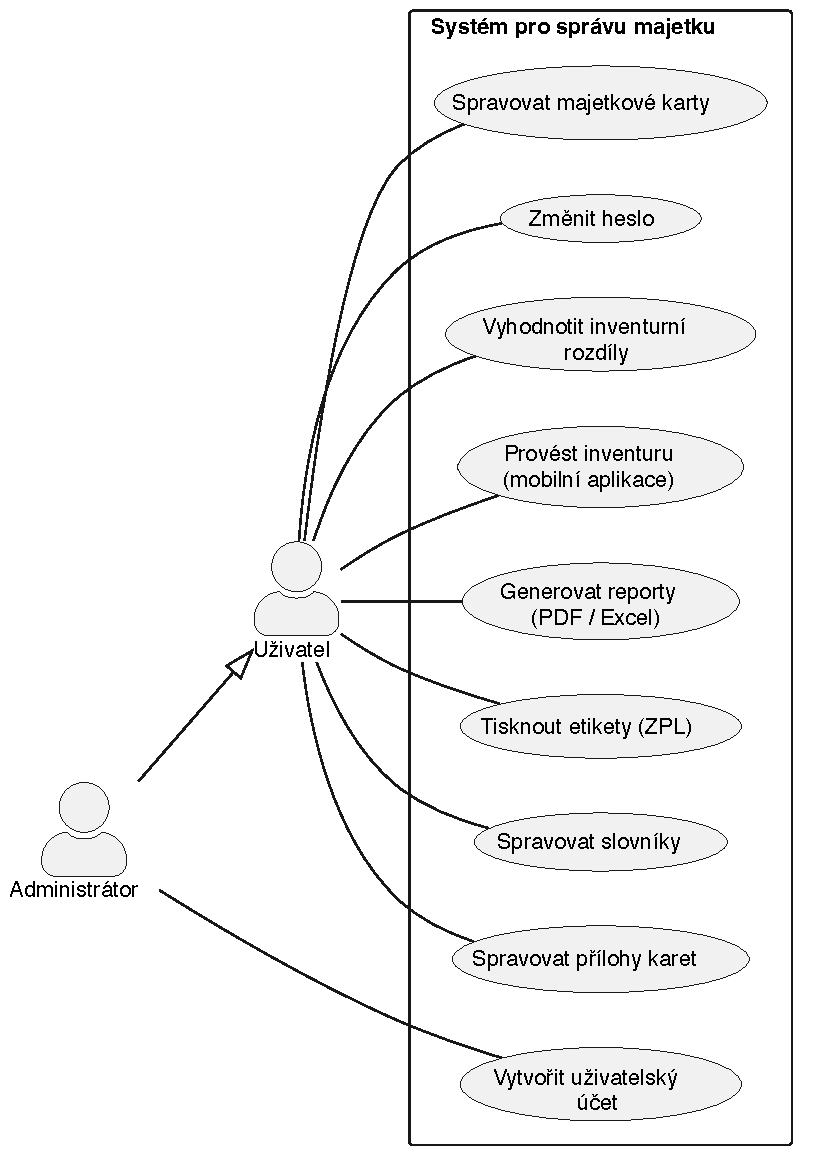
\includegraphics[width=0.65\textwidth]{images/use-case-diagram.pdf}
	\caption{Diagram případů užití}\label{fig:use-case-diagram}
\end{figure}

Diagram případů užití je znázorněn na obrázku~\ref{fig:use-case-diagram}. Následující podsekce popisují klíčové scénáře. U~všech scénářů se předpokládá, že uživatel je přihlášen.

\subsection{Správa majetkové karty}

\textbf{Cíl:} Vytvořit, upravit nebo duplikovat majetkovou kartu v~evidenci.

\begin{enumerate}
	\item Systém zobrazí seznam majetkových karet v~levém panelu.
	\item Uživatel klikne na tlačítko pro vytvoření nové karty.
	\item Systém zobrazí formulář s~povinnými poli (název, umístění, skupina, datum pořízení) a~volitelnými poli.
	\item Uživatel vyplní údaje a~potvrdí uložení.
	\item Systém ověří správnost zadaných dat (povinná pole, formáty) a~vytvoří kartu.
\end{enumerate}

\textit{Alternativní scénář:} Uživatel vybere existující kartu ze~seznamu, upraví její atributy a~uloží změny. Pro rychlé zadávání podobného majetku může existující kartu duplikovat.

\subsection{Tisk etiket}

\textbf{Cíl:} Vytisknout etikety s~Data Matrix kódy pro vybrané karty majetku nebo místnosti.

\begin{enumerate}
	\item Uživatel vyhledá požadované karty pomocí fulltextového vyhledávání nebo filtrů a~klikne na tlačítko tisku.
	\item Systém vygeneruje ZPL etikety a~odešle je na tiskárnu Zebra prostřednictvím cloudového tisku, případně nabídne ke~stažení jako \texttt{.zpl} soubor pro lokální tisk.
	\item Uživatel nalepí vytištěné etikety na příslušné položky majetku. Etikety místností se lepí na zárubně dveří.
\end{enumerate}

\subsection{Sběr inventurních dat}

\textbf{Cíl:} Zaznamenat skutečné umístění majetku v~terénu pomocí mobilní aplikace.

\begin{enumerate}
	\item Pracovník vyžádá stažení aktuálních dat ze~serveru.
	\item Systém ověří připojení, autentizuje se vůči serveru a~uloží karty a~lokace do~lokální databáze.
	\item Pracovník naskenuje Data Matrix kód místnosti.
	\item Systém nastaví aktuální umístění a~zobrazí jeho název.
	\item Pracovník postupně skenuje kódy majetku v~dané místnosti.
	\item U~každé naskenované karty systém barevně signalizuje, zda karta evidenčně patří do~aktuálního umístění (zelená), jiného umístění (oranžová), nebo nebyla v~databázi nalezena (červená), a~ukládá záznam o~naskenování do~lokální databáze.
	\item Po dokončení místnosti pracovník přejde do~další a~opakuje kroky 3--6.
	\item Pracovník vyžádá nahrání inventurních dat na server.
	\item Systém odešle všechny lokální záznamy hromadným požadavkem a~potvrdí úspěch.
\end{enumerate}

\subsection{Vyhodnocení inventury}

\textbf{Cíl:} Porovnat evidovaný stav majetku se skutečným a~promítnout změny do~databáze.

\begin{enumerate}
	\item Systém zobrazí seznam všech karet s~barevným rozlišením:
	\begin{itemize}
		\item \textit{Shodné} (zelená) -- evidované umístění odpovídá skutečnosti.
		\item \textit{Upozornění} (oranžová) -- karta nalezena na jiném umístění.
		\item \textit{Chybné} (červená) -- karta nebyla při inventuře naskenována.
	\end{itemize}
	\item U~karet se~stavem \uv{upozornění} uživatel zvolí: přijmout skutečné umístění, ponechat evidované, nebo majetek vyřadit. U~karet se~stavem \uv{chybné} lze ponechat evidované umístění nebo majetek vyřadit. U~shodných karet lze rovněž zvolit vyřazení.
	\item Po rozhodnutí u~všech karet s~nesouladem uživatel potvrdí promítnutí změn.
	\item Systém ověří, že každá karta se~stavem \uv{chybné} má zvolenou akci a~každá vyřazovaná karta má vyplněné datum a~způsob vyřazení. Poté aplikuje změny do~databáze.
\end{enumerate}

\subsection{Generování reportů}

\textbf{Cíl:} Vygenerovat přehledovou sestavu majetku pro potřeby účetnictví.

\begin{enumerate}
	\item Uživatel zvolí typ sestavy (podle skupiny majetku, podle místnosti, nebo pro konkrétní kartu).
	\item Uživatel vyplní parametry sestavy:
		\begin{itemize}
			\item \textit{podle skupiny majetku} -- konkrétní skupinu (nebo všechny skupiny) a~rozhodný den, ke~kterému se sestava generuje;
			\item \textit{podle místnosti} -- konkrétní místnost (číselník umístění);
			\item \textit{pro konkrétní kartu} -- identifikátor karty.
		\end{itemize}
	\item Systém vygeneruje PDF dokument a~zobrazí jej přímo v~prohlížeči.
	\item Uživatel si může sestavu stáhnout nebo vytisknout.
\end{enumerate}

\medskip

Vazba mezi případy užití a~funkčními požadavky je shrnuta v~tabulce~\ref{tab:uc-fr-mapping}.

\begin{table}[H]\centering
\renewcommand{\arraystretch}{1.3}
\caption{Mapování případů užití na funkční požadavky}\label{tab:uc-fr-mapping}
\begin{tabular}{l|l}
	\textbf{Případ užití} & \textbf{Plněné funkční požadavky} \tabularnewline \hline
	Správa majetkové karty & F-01 -- F-07 \tabularnewline
	Tisk etiket            & F-09 -- F-11 \tabularnewline
	Sběr inventurních dat  & F-16 -- F-20 \tabularnewline
	Vyhodnocení inventury  & F-21 -- F-24 \tabularnewline
	Generování reportů     & F-12 -- F-15 \tabularnewline
\end{tabular}
\end{table}


